\newpage

\section{Descrizione architettura}
\label{descrizione_architettura}
\subsection{Introduzione}
Il prodotto \progetto{}, creato dal \glo{Gruppo}{gruppo} \zephyrus{}, sarà integrabile nell'attuale applicazione del proponente \riskapp{}.
\\Per esporre l'architettura dell'applicazione si procederà con approccio top-down, partendo cioè da una visione generale delle componenti che distinguono il sistema, per poi analizzare in dettaglio la conformazione di tali componenti.
%Molte scelte architetturali sono state dettate dal requisito dell'integrabilità richiesto dal proponente. 
\\Il sistema attuale di \riskapp{} presenta un'architettura client-server.
\subsection{Server}
\progetto{} si connetterà al server di \riskapp{} esclusivamente utilizzando le \glo{API}{API} REST fornite dal proponente stesso e riportate in questa sezione. Il gruppo non ha quindi accesso all'implementazione del server di \riskapp{}.
\subsubsection{Chiamate REST}
L'interfaccia REST proposta da \riskapp{} fornisce l'accesso alle seguente entità:
\begin{itemize}
	\item Customer
	\item Graph
	\item \glo{Asset}{Asset}
	\item Node
	\item Edge
\end{itemize}
Per ognuna di queste è possibile fare una chiamata REST usando i verbi http. (GET, OPTION, POST, PUT, UPDATE, DELETE)\\\\
Tutte queste entità sono identificate univocamente da uno uuid formato come una stringa di cifre esadecimali con la seguente struttura:
\begin{center}
	XXXXXXXX-XXXX-XXXX-XXXX-XXXXXXXXXXXX
\end{center}
Il verbo OPTION viene utilizzato all'interno del server di Riskapp per ottenere informazioni sulla struttura (nomi dei campi dati e relativi tipi di dato) delle entità ricevute a seguito di una chiamata GET o necessarie per le chiamate POST e PUT.
Inoltre per determinati campi, la chiamata OPTION restituisce tutti i possibili valori, nel caso siano limitati al lato server, per il campo stesso.

\paragraph{Customer}
\begin{itemize}
	\item \textbf{descrizione:} l'entità customer contiene le informazioni del cliente;
	\item \textbf{chiamata:} /mitsuko/v01/customer/<uuid>/uuid/
	\begin{itemize}\item \textbf{operazioni utilizzate:} GET.\end{itemize}
\end{itemize}

\paragraph{Graph}
\begin{itemize}
	\item \textbf{descrizione:} l'entità grafo proposta da \riskapp{} contiene le informazioni relative al processo produttivo e ai suoi \glo{Nodo}{nodi};
	\item \textbf{chiamata:} /mitsuko/v01/graph/<uuid>/uuid/
	\begin{itemize}\item \textbf{operazioni utilizzate:} GET.\end{itemize}
\end{itemize}

\paragraph{Asset}
\begin{itemize}
	\item \textbf{descrizione:} l'entità asset rappresenta un asset del cliente con le relative informazioni;
	\item \textbf{chiamata:} /mitsuko/v01/customer/<uuid>/asset/new/
	\begin{itemize}\item \textbf{operazioni utilizzate:} POST.\end{itemize}
	\item \textbf{chiamata:} /mitsuko/v01/asset/<uuid>/uuid/
	\begin{itemize}\item \textbf{operazioni utilizzate:} GET, PUT, OPTIONS, UPDATE, DELETE.\end{itemize}
\end{itemize}

\paragraph{Node}
\begin{itemize}
	\item \textbf{descrizione:} l'entità node rappresenta un elemento di interesse strategico all'interno di un asset;
	\item \textbf{chiamata:} /mitsuko/v01/graph/<uuid>/node/new/
	\begin{itemize}\item \textbf{operazioni utilizzate:} POST.\end{itemize}
	\item \textbf{chiamata:} /mitsuko/v01/node/<uuid>/uuid/
	\begin{itemize}\item \textbf{operazioni utilizzate:} GET, PUT, OPTIONS, UPDATE, DELETE.\end{itemize}
\end{itemize}

\paragraph{Edge}
\begin{itemize}
	\item \textbf{descrizione:} l'entità edge rappresenta un collegamento fra due nodi;
	\item \textbf{chiamata:} /mitsuko/v01/graph/<uuid>/edge/new/
	\begin{itemize}\item \textbf{operazioni utilizzate:} POST.\end{itemize}
	\item \textbf{chiamata:} /mitsuko/v01/edge/<uuid>/uuid/
	\begin{itemize}\item \textbf{operazioni utilizzate:} GET, PUT, OPTIONS, UPDATE, DELETE.\end{itemize}
\end{itemize}

\newpage
\subsection{Client}
Il proponente ha fornito l'ambiente di sviluppo contenente la loro attuale applicazione, denominata in figura come "\riskapp", su cui il gruppo potrà integrare \progetto. Il prodotto sarà sviluppato come una single-page accessibile cliccando sulla scheda di menu "Process and analysis".

\subsubsection{Design architetturale di DeGeOP}
E' stato scelto di utilizzare il design architetturale Redux (per maggiori informazioni su questo pattern, si veda l'appendice \ref{dp_redux}).
Per una migliore gestione e uso di questo pattern si è deciso di rafforzare l'uso classico di Redux, incapsulando le varie componenti in una struttura a classi.
Rispetto all'architettura base, ovvero Redux, sono quindi presenti altre componenti:
\begin{itemize}
	\item \textbf{ActionCreators:} struttura il cui compito è creare le "azioni", ossia le operazioni che si occupano di interagire con lo \glo{Store}{store}. Le actions come fornite da Redux permettono di definire azioni potenzialmente invalide o la cui esecuzione potrebbe portare ad errori. È quindi nata la necessità di incapsulare il concetto di azione e devolvere il compito della sua creazione ad una \glo{Componente}{componente} propria;
	\item \textbf{\glo{Reducer}{Reducer}:} classe di utilità che accetta \glo{Action}{action} generiche e le reindirizza alle giuste implementazioni per gestire l'azione in analisi. Anche in questo caso l'incapsulazione è stata adottata per fornire una migliore interfaccia di utilizzo dei reducer.
\end{itemize}

\begin{figure}[H]
	\label{diagramma_architettura}
	\centering
	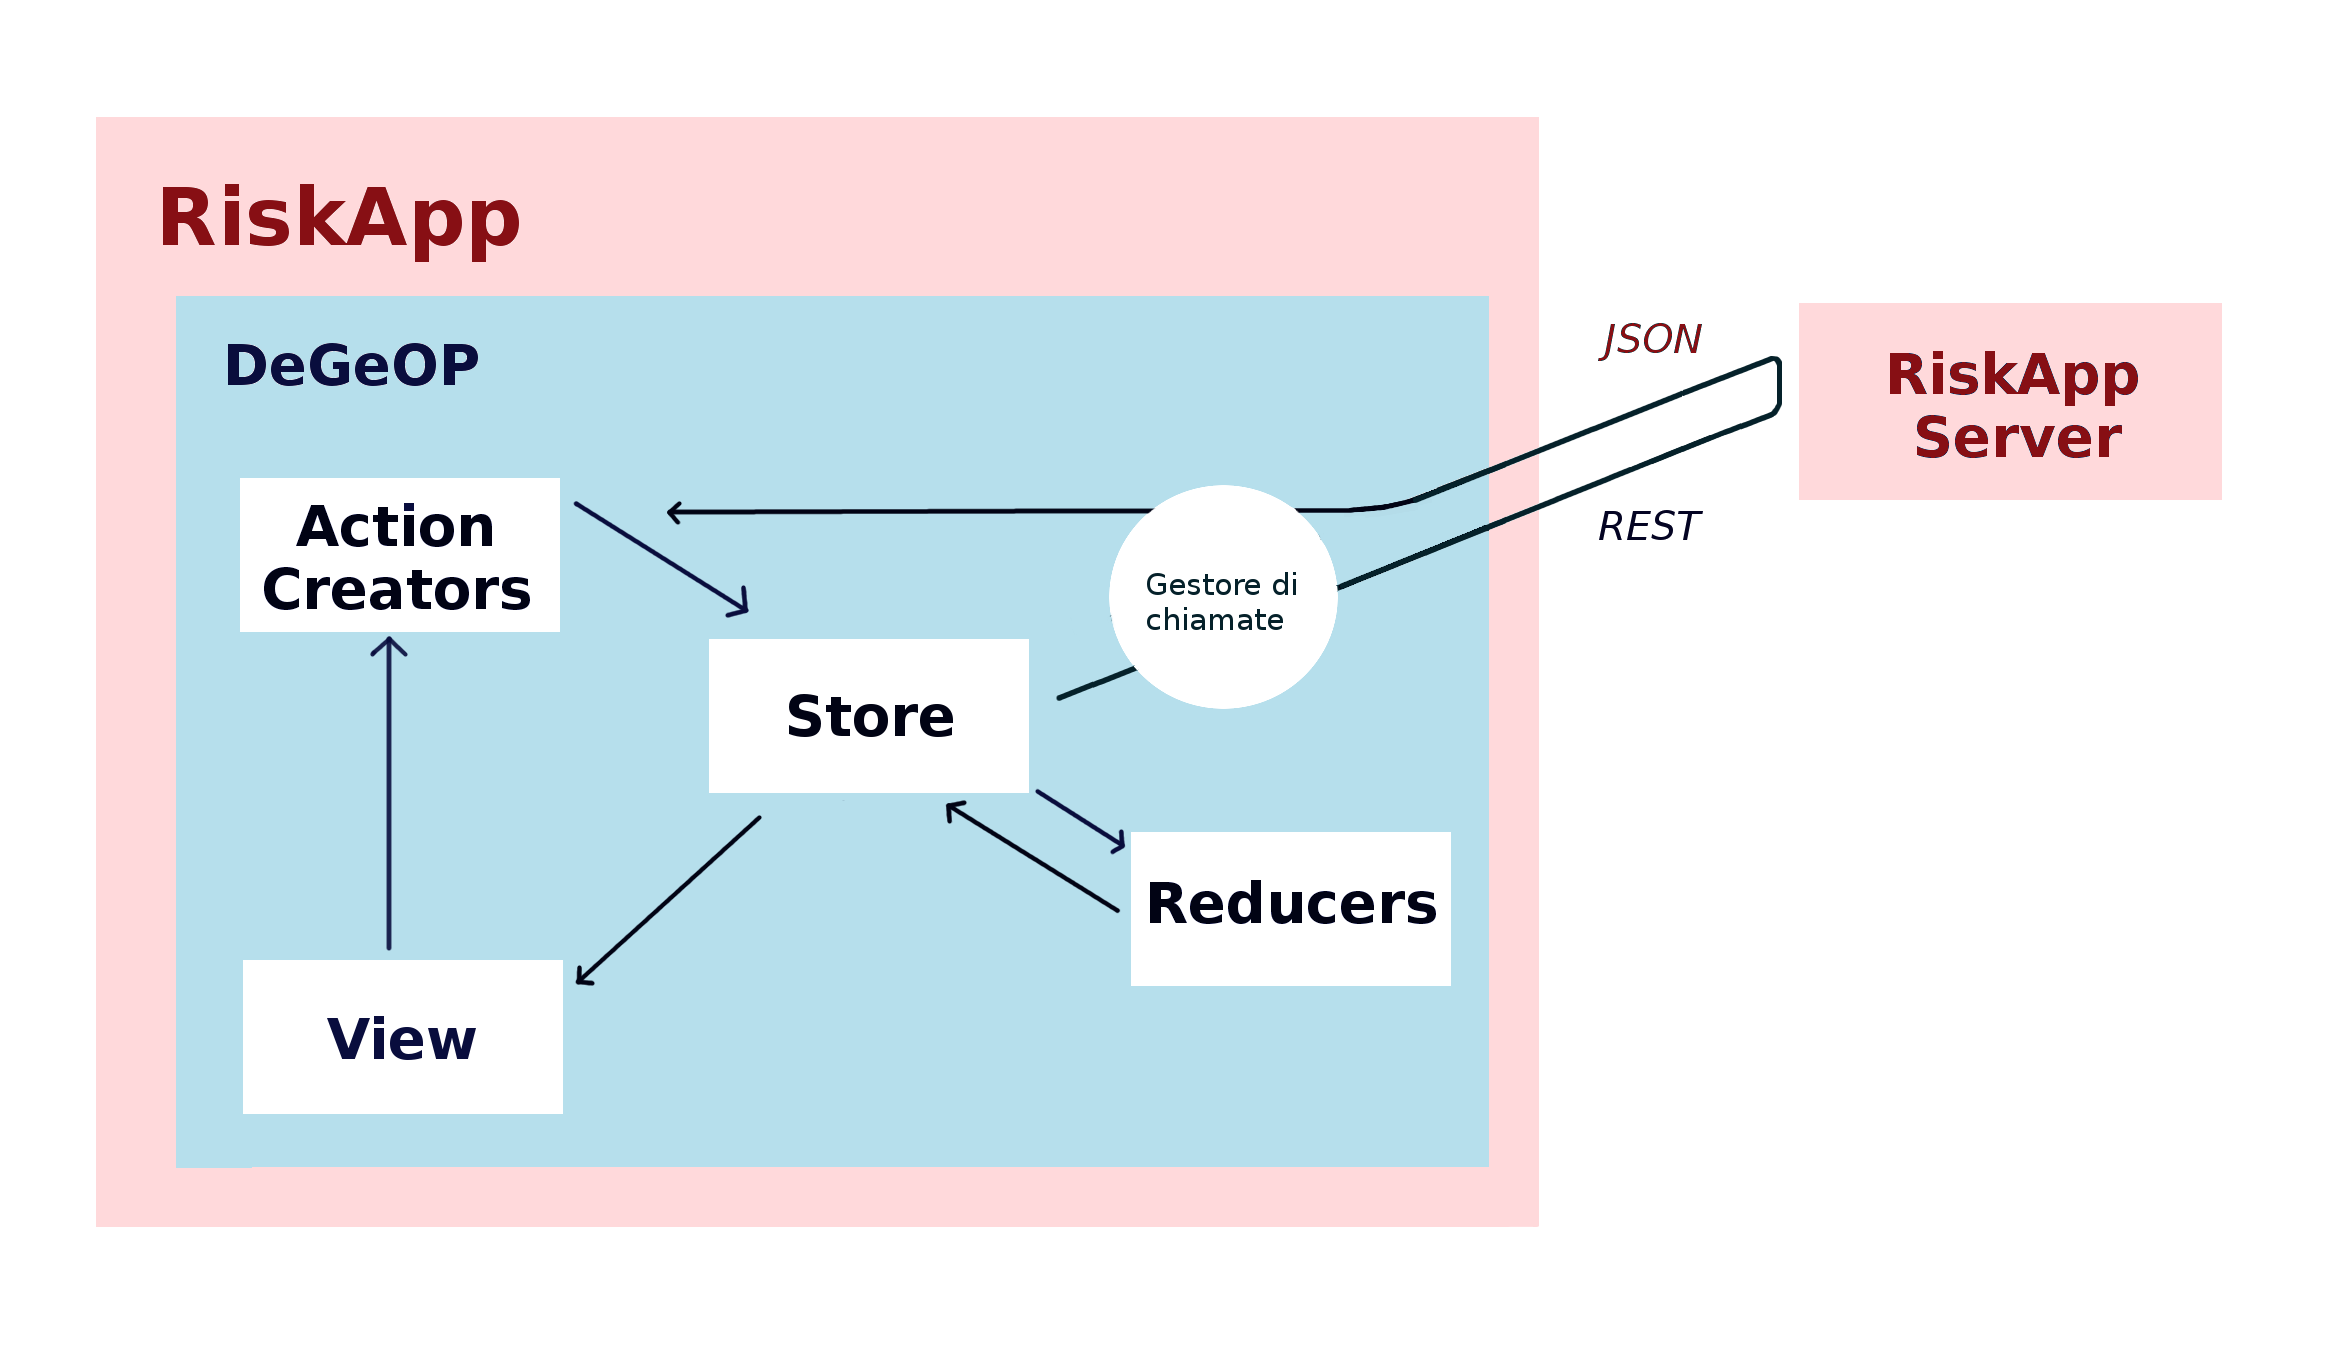
\includegraphics[width=\textwidth]{img/ArchitetturaBase.png}
	\caption{Architettura di base}
\end{figure}


